\chapter{Web-based E-learning System and SCORM}
\thispagestyle{empty}
In this chapter, some technology related to E-learning system is explained, which paved the way for utilizing them in this project.
\section{Learning Management Systems}
A Learning Management System (LMS) is a software package that is typically accessible via the Internet and is used to manage one or more courses to 
one or more learners. In other words, an LMS allows learners to authenticate themselves, register for courses, access learning content, take 
assignments, and then store the learners’ grade records \cite{lms}. Apparently, this model is based on physical administration process.
\section{Learning Content Management Systems}
An Learning Content Management System (LCMS) is a development of the LMS. It is a multi-tier environment where learning materials developers may 
create, store, reuse, manage, and deliver digital learning content from a central content repository \cite{lcms}. To some extent, LCMS can be treated 
as one combination of the original LMS and Authoring Tools, which will be explained immediately.
\section{Authoring Tools}
Authoring tools are software applications used to develop E-learning products. They generally include the capabilities to create, edit, review, test, 
and configure E-learning packages. These tools support learning, education, and training by using distributed E-learning system that is 
cost-efficient to produce, and that facilitates incorporating effective learning strategies and delivery technologies into the E-learning system. 
Authoring tools themselves are not SCORM-certified, but many are designed to create SCORM compliant E-learning course materials \cite{at}.

Since it is very convenient to use LCMS, LMS and authoring tools do not appear as standalone applications any more. In this project, the term ``LMS'' 
is used, even though, in fact, ``LCMS'' is concerned.
\section{History of SCORM}
In the late 1990s, as computer was getting more and more popular, everyone was using computer in their daily life and work. The United States 
Department of Defense realized that they were procuring the same training content many times over and over again, but could not reuse it across 
departments, because each department had its own Learning Management System. In those days, each LMS had its own proprietary content format, which 
discouraged content sharing. In 1999 an executive ordered a small research laboratory, Advanced Distributed Learning(ADL), to ``develop common 
specifications and standards for E-learning.'' Rather than starting from scratch, ADL harmonized the work of existing standards organizations like 
the Aviation Industry Computer-Based Training Committee (AICC) \cite{aicc}, IMS \cite{ims} and the IEEE Learning Technology Standards Committee 
(LTSC) \cite{ltsc} into a cohesive reference model, which becomes SCORM later. SCORM was released in 2001 and was quickly adopted by both government 
and industry. Today it is the de facto standard for E-learning interoperability \cite{history_of_scorm}.
\section{SCORM Variation}
\label{sec:scorm_variation}
With the technology of Internet and computer gets more and more mature, people has improved SCORM so that it could adapt to various situations. At 
present, there are three major players on the stage.
\begin{itemize}
	\item SCORM 2004 \\
		This is the current version. It is based on new standards for API and content object-to-runtime environment communication, with many 
		ambiguities of previous versions resolved. It contains ability to specify adaptive sequencing of activities that use the content objects, and 
		the ability to share and use information about success status for multiple learning objectives or competencies across content objects and 
		across courses for the same learner within the same learning management system \cite{scorm_overview}.
	\item SCORM Cloud \\
		Using SCORM Cloud, learners can be reached where they are rather than forcing them to go to the LMS. In addition to supplying best of class 
		SCORM, SCORM Cloud serves as a connection point between one LMS and the rest of the Internet \cite{scorm_cloud}.
	\item Tin Can \\
		Over the last decade, two phenomena have happened. First, as the adoption of SCORM soared, people wanted to utilize it in new ways, ways that 
		stretched the limits of what SCORM was designed to do. Second, technology has evolved at a rapid pace. In comparison with present 
		technologies, the current SCORM structure is antiquated and inadequate. Both of these trends demand the need for a more modern and powerful 
		communication framework \cite{tin_can}.
\end{itemize}

The biggest advantage of SCORM Cloud over SCORM 2004 is that it does not require users to go to the LMSs. Instead, users can be connected and tracked 
anywhere in the web. In this case, users are asked to come to the LMS, and take the test in this LMS, so SCORM 2004 suffices. The weakest point of 
Tin Can is that this project hasn't finished yet. According their announcement \cite{tin_can}, this project consists of three phases, and they are 
still in the first phase when this project is conducted. Therefore, the most appropriate solution for this case is SCORM 2004. In the following, 
SCORM 2004 is introduced.
\section{SCORM 2004}
SCORM specifiers that content should:
\begin{itemize}
	\item
		Be packaged in a ZIP file.
	\item
		Have one XML to describe the package
	\item
		Communicate with the LMS via JavaScript.
	\item
		Define sequence using rules in XML.
\end{itemize}
SCORM consists of three sub-specifications:
\begin{itemize}
	\item
		The Content Packaging section specifies how content should be packaged and described. It is based primarily on XML. The content should be 
		packaged in a ZIP file.
	\item
		The Run-Time section specifies how content should be launched and how it communicates with the LMS. It is based primarily on ECMAScript 
		(JavaScript). The LMS should launch content in a web browser, either in a new window or in a frameset.
	\item
		The Sequencing section specifies how the learner can navigate between parts of the course. It is defined by a set of rules and attributes 
		written in XML.
\end{itemize}

Considering the particular tasks in this project, content packaging is focused.
\section{The SCORM Content Aggregation Model}
The SCORM Content Aggregation Model (CAM) represents a learning-taxonomy neutral way for designers and implementers of instruction to aggregate 
learning resources for the purpose of delivering a desired learning experience \cite{cambook}.

The SCORM CAM consists of the following:
\begin{itemize}
	\item
		Content Model: Define the content components of a learning experience.
	\item
		Content Packaging: How to structure and exchange learning content.
	\item
		Metadata: A mechanism for describing specific instances of the components of the content model.
	\item
		Sequencing and Navigation: A rule-based model for defining a set of rules that describes the intended sequence and ordering of activities.
\end{itemize}
In this project, only Content Model and Content Packaging are used. In the following, they are explained thoroughly.
\begin{figure}[t]
	\begin{center}
		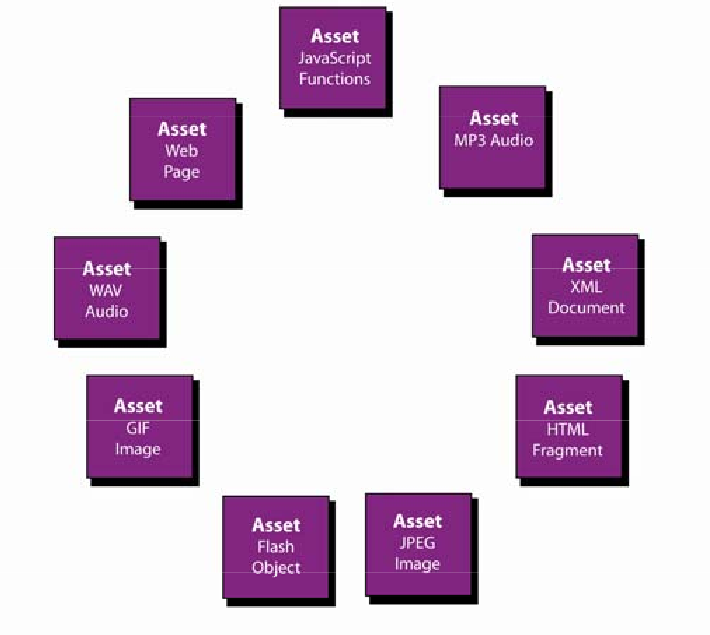
\includegraphics[scale=0.4]{asset.png}
	\end{center}
	\caption{Examples of asset \cite{cambook}.}
	\label{fig:asset}
\end{figure}
\begin{figure}[t]
	\begin{center}
		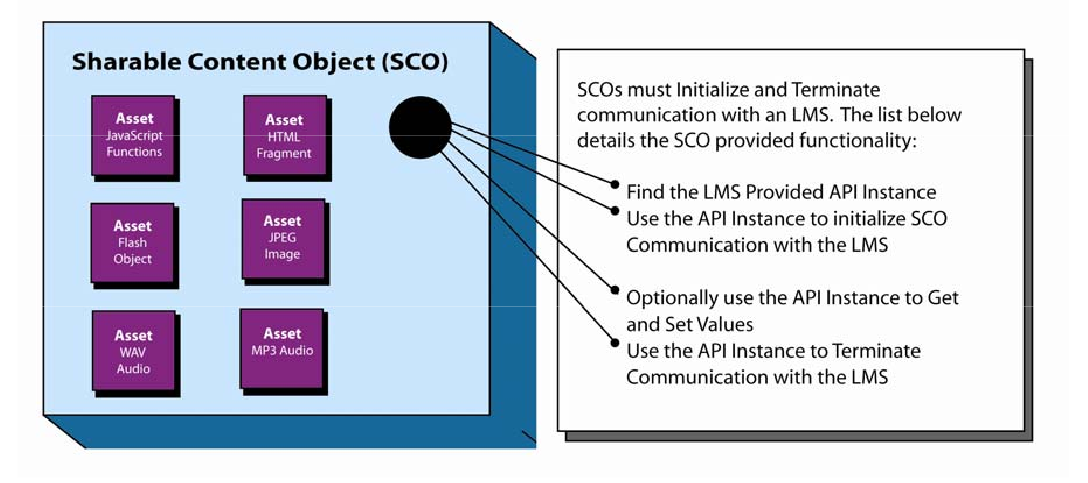
\includegraphics[scale=0.4]{sco.png}
	\end{center}
	\caption{Conceptual markup of a SCO \cite{cambook}.}
	\label{fig:sco}
\end{figure}
\subsection{Content Model}
The SCORM Content Model explains the SCORM components used to construct a learning experience from learning resources. The content model also defines 
how these low level sharable, learning resources are aggregated and organized into higher-level units of instruction. The SCORM Content Model is made 
up of assets, sharable content objects (SCOs), activities, a content organization and content aggregations \cite{cambook}.
\begin{itemize}
	\item Asset \\
		The asset is the basic building block of a learning resource. Assets are an electronic representation of media, such as text, images, sound, 
		assessment objects or any other piece of data that can be rendered by a Web client and presented to a learner.

		Typical examples of asset are shown in Figure~\ref{fig:asset}.
	\item SCO \\
		A SCO is a collection of one or more assets that represent a single launchable learning resource that uses the SCORM RTE to communicate with 
		an LMS. Figure~\ref{fig:sco} illustrate the markup of SCO. The only difference between a SCO and an asset is that the SCO communicates with 
		LMS using javascript.
	\item Activities \\
		A learning activity may be loosely described as a meaningful unit of instruction; it is conceptually something the learner does while 
		proceeding through instruction.

		The activities represented in a content organization may consist of other activities (sub-activities), which may themselves consist of other 
		activities. There is no limit to the number of levels of nesting for activities. Activities that do not consist of other activities (leaf 
		activities) will have an associated learning resource (SCO or asset) that is used to perform the activity.
	\item Content Organization \\
		A content organization is a representation or map that defines the intended use of the content through structured units of instruction 
		(activities). The map shows how activities relate to one another. In other words, it represents the sequencing information.

		The LMS is responsible for interpreting the sequencing information described in the content organization and applying sequencing behaviors to 
		control the actual sequence of the learning resources at run-time.
	\item Content Aggregation \\
		Content aggregation can be used as both an action and as a way of describing a conceptual entity. Sometimes, this term is loosely used to 
		describe content package.
\end{itemize}
\begin{figure}[t]
	\begin{center}
		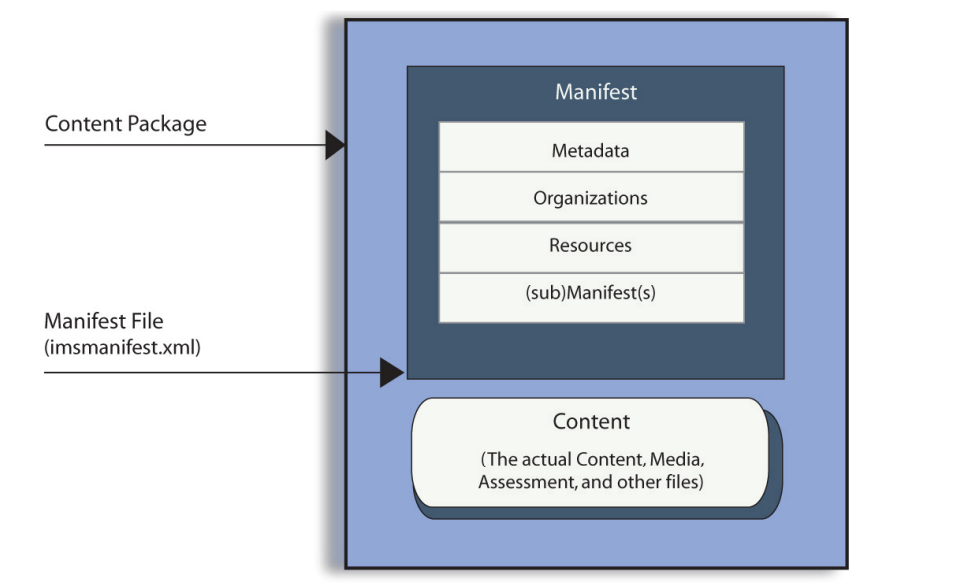
\includegraphics[scale=0.4]{contentPackaging.png}
	\end{center}
	\caption{Components of a content package \cite{cambook}.}
	\label{fig:components_of_a_content_package}
\end{figure}
\begin{figure}[t]
	\begin{center}
		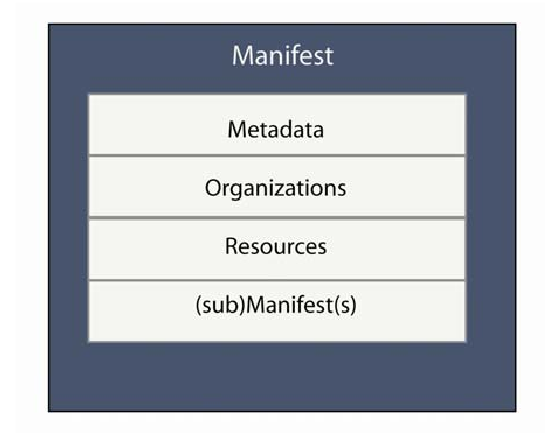
\includegraphics[scale=0.4]{manifest.png}
	\end{center}
	\caption{Components of a Manifest \cite{cambook}.}
	\label{fig:components_of_a_Manifest}
\end{figure}
\subsection{Content Packaging}
The purpose of the content package is to provide a standardized way to exchange learning content between different systems or tools.
\subsubsection{Content Package Component}
A content package contains two major components \cite{cambook}, as presented in Figure~\ref{fig:components_of_a_content_package} and described in 
below:
\begin{itemize}
	\item A special XML document describing the content structure and associated resources of the package called the manifest file (imsmanifest.xml). 
		A manifest is required to be present at the root of the content package.
	\item The content (i.e., physical files) making up the content package.
\end{itemize}
\subsubsection{Components of a Manifest}
The general rule is that one single manifest file exists in the root directory, describing this package. At present, ADL recommends not to use 
(sub)manifests until the completion of the corresponding work. The manifest consists of four major components \cite{cambook}, as presented in 
Figure~\ref{fig:components_of_a_Manifest} and explained in below:
\begin{itemize}
	\item Metadata: Data describing the content package as a whole, which enables the search and discoverability of the package itself.
	\item Organizations: Contains the content structure or organization of the learning resources making up a stand-alone unit or units of 
		instruction. A definition of sequencing intent can be associated with the content structure.
	\item Resources: Defines the learning resources bundled in the content package.
	\item (sub)Manifest(s): Describes any logically nested units of instruction (which can be treated as stand-alone units).
\end{itemize}
This section will be reviewed in detail with one example in next chapter.
\subsubsection{SCORM Content Package Application Profiles}
SCORM Content Package Application Profiles describe how the IMS Content Packaging Specification will be applied within the overall context of SCORM. 
There are currently two SCORM Content Package Application Profiles, which describe how to package CAM components: \cite{cambook}
\begin{itemize}
	\item Resource Content Packages \\
		The SCORM Resource Content Package Application Profile defines a mechanism for packaging assets and SCOs without having to provide any 
		organization, learning context or curricular taxonomy.
	\item Content Aggregation Content Packages \\
		Its main purpose is to be used to deliver content to an end user (i.e., typically through an LMS).
\end{itemize}
